% Two-page findings report on the latent-token clustering project.
% Build:  cd report && pdflatex report.tex && pdflatex report.tex
% Minimal TeX install on this box: geometry/graphicx/amsmath/url are available
% (no booktabs/algorithm/xcolor/caption, and the Times metrics are missing), so
% tables use \hline, the pseudocode box is hand-rolled and the font is Computer
% Modern.  References are plain \thebibliography (no natbib/biblatex needed).
% Page 3 is an appendix: two full-width figure* floats plus the reference list.
\documentclass[10pt,twocolumn]{article}
\usepackage[a4paper,margin=1.6cm,columnsep=0.7cm]{geometry}
\usepackage{amsmath,amssymb}
\usepackage{graphicx}
\usepackage{url}
\usepackage{multicol}

% ---- measured numbers from the k-means / k-center baseline sweep ----
% (v13-v15 = k-means d=0 seeds 0/1/2; v16 = k-center seeds 0/1/2; filled in
% from the run logs once the sweep finishes)
\newcommand{\kmobj}{5021.1}              % best k-means obj/token (v14, seed 1)
\newcommand{\kmspread}{0.05\%}           % k-means seed spread (5023.8 vs 5021.1)
\newcommand{\kmresid}{83.7\%}            % k-means residual as % of total variance
\newcommand{\kmnmi}{0.31}                % NMI(v14 k-means, v6); v13 gives 0.31 too
\newcommand{\kmpca}{2270}                % post-hoc d=64 PCA residual of k-means partition (37.8%)
\newcommand{\kcobj}{9744.2}              % best k-center obj/token (seed 1)
\newcommand{\kcresid}{162\%}             % k-center residual as % of total variance
\newcommand{\kcspread}{40.8\%}           % k-center obj spread (9744 vs 13723)
\newcommand{\kcrad}{146.4}               % k-center minimax radius (best seed)
\newcommand{\kcminmax}{196 to 84.9M}     % k-center size min/max (seed 1)
% ---- seed agreement: the two NMI measurements are on DIFFERENT objects ----
% token level (partition_nmi.py, 86M rows): v6/v7 .683, v6/v8 .688, v7/v8 .693,
%   chance (size-preserving shuffle) 2e-05.
% per-cell dominant map (12,288 rows): .716/.727/.725, chance 0.130 +/- 0.001.
% An earlier draft quoted "0.68 to 0.72 (chance 0.13)", which mixed the two.
\newcommand{\nmitok}{0.68 to 0.69}      % token-level seed-to-seed NMI
\newcommand{\nmimap}{0.72}              % per-cell dominant-map seed-to-seed NMI
\newcommand{\nmimapchance}{0.13}        % chance level for the per-cell map
\newcommand{\cellspan}{12.4}            % per-cell mean residual max/min (3386/273)
% ---------------------------------------------------------------------

\setlength{\parskip}{0pt}
\setlength{\textfloatsep}{8pt}
\setlength{\floatsep}{8pt}
\setlength{\intextsep}{8pt}
\setlength{\abovecaptionskip}{5pt}
\raggedbottom

\begin{document}

\twocolumn[{%
\begin{center}
{\LARGE Subspace Structure of WeatherGenerator Latent Tokens\par}
\vspace{5pt}
{\large Clustering methods and findings\par}
\vspace{6pt}
Paulin Saher, September 2026
\end{center}
\vspace{4pt}
\noindent\rule{\textwidth}{0.4pt}
\vspace{2pt}
\begin{quote}
\small\textbf{Abstract.}
We analyse the 2048-dimensional tokens the WeatherGenerator encoder produces
for nine years of ERA5 states (160\,M tokens). A K-subspaces clustering, a
variant of k-means in which each cluster is a 64-dimensional affine subspace
instead of a single centre point, explains 68.5\% of token variance with
K=128 clusters. Plain k-means, run as a baseline on the same data, captures
almost none of the structure inside each regime and lands on a different
partition. The clusters turn out to be climate regimes. They are
geographically coherent, a minority of them carries a strong seasonal cycle,
and the El Ni\~no winters stand out in the central Pacific. Several of the
largest residual outliers of the fit coincide with documented extreme weather
events, so the encoder does capture extremes.
\end{quote}
\vspace{4pt}
}]

\section{Introduction}
The WeatherGenerator (WGen) model~\cite{wgen} encodes each 6-hourly ERA5
atmospheric state~\cite{era5} into 12{,}288 tokens, one per HEALPix grid
cell~\cite{healpix}, with 2048 dimensions each.
This project analyses the encoder output for all 13{,}021 available states,
covering 2014-01-01 00:00 to 2022-11-30 00:00 UTC. Two questions drove the
analysis, in order of importance. First, can we tell from the latents whether
the model actually encodes extreme weather events, meaning that real extremes
show up as outliers? Second, how does the model handle spatial and temporal
structure? Clustering answers both at once. It yields a regime label and a
residual per cell and timestep, and the residual is the outlier score.

\section{Methodology}
\textbf{Data.} 13{,}021 encoder states of shape $[12{,}288 \times 2048]$,
1.2\,TB in total. All clustering runs use the same fixed random sample of
7{,}000 states times all cells, 86\,M tokens. Evaluation replays the fitted
model on the full dataset or on held-out states.

\textbf{K-subspaces}~\cite{kplane,qflat}. Cluster $j$ is not a centre $\mu_j$ but an affine
subspace $(\mu_j, U_j)$ with orthonormal basis $U_j \in
\mathbb{R}^{2048\times 64}$. The difference to k-means lies in the assignment
step. A token $x$ is assigned by its distance to the whole subspace,
\begin{equation}
r_j(x) \;=\; \underbrace{\|x-\mu_j\|^2}_{\text{k-means distance}}
\;-\; \underbrace{\|U_j^\top (x-\mu_j)\|^2}_{\text{part the subspace explains}},
\label{eq:resid}
\end{equation}
the centre distance minus what the cluster's own principal directions account
for. A token far from $\mu_j$ along directions in which the cluster normally
varies still belongs to it. The update step is exact PCA per cluster.

\medskip
\noindent\fbox{\parbox{0.965\columnwidth}{\small
\textbf{Algorithm} (K-subspaces, $K{=}128$, $d{=}64$, $D{=}2048$)\\[2pt]
\textbf{init:} $\mu_j \leftarrow K$ random tokens, $U_j \leftarrow 0$\\
\textbf{repeat}, at most 25 times, until $<$0.1\% of labels change:\\
\hspace*{1em}1. assign each token to the nearest subspace:\\
\hspace*{2em}for every token $x$ and cluster $j$:\\
\hspace*{3em}$z \leftarrow U_j^\top(x-\mu_j)$ \hfill{\footnotesize coords inside the subspace}\\
\hspace*{3em}$r_j(x) \leftarrow \|x-\mu_j\|^2 - \|z\|^2$ \hfill{\footnotesize Eq.~\ref{eq:resid}}\\
\hspace*{2em}$\mathrm{label}(x) \leftarrow \arg\min_j r_j(x)$\\
\hspace*{1em}2. refit each cluster to its members:\\
\hspace*{2em}$\mu_j \leftarrow$ mean of its tokens\\
\hspace*{2em}$U_j \leftarrow$ top-$d$ eigenvectors (PCA) of their covariance\\
\hspace*{1em}3. split the largest cluster to replace any collapsed one
}}
\medskip

Setting $d=0$ turns the same code into plain k-means~\cite{lloyd}, the first
baseline. Greedy k-center~\cite{gonzalez}, which minimises the largest distance
to a centre, is the second. A soft-assignment variant (an MPPCA
mixture~\cite{mppca}) was fitted afterwards and is used only to quantify
per-token uncertainty. One fit takes about two and a half hours on two A40
GPUs. Results were checked on held-out states, across three random
restarts, and against an independent run at $K{=}256$ merged back to 128.

\section{Results}

\subsection{Fit quality and baselines}
At $K{=}128$, $d{=}64$ the fit splits token variance into 8.4\% between
cluster centres, 60.1\% captured inside the subspaces, and 31.5\% residual.
Almost all structure is therefore inside the clusters, not between their
centres. On held-out dates the residual fraction is also 31.5\%, meaning no
overfitting.

Table~\ref{tab:methods} compares the methods. K-means leaves \kmresid{} of
the variance unexplained and finds a different
partition (NMI \kmnmi{} against the subspace one). Even when its clusters are
given the same 64-dimensional PCA fit after the fact, the residual is still
\kmpca{} per token against 1877 to 1892 for the subspace runs. Re-assigning
tokens under the fitted subspace model by centre distance alone changes 57\%
of the labels and adds 20\% residual. K-center degenerates. Greedy selection
anchors nearly all centres on outliers. One cluster ends up with 98.8\% of
all tokens (sizes \kcminmax) and the objective lands above the total
variance, worse than a single global centroid. Only its minimax radius is
stable across seeds (146 to 148).

\begin{table}[t]
\centering\small
\caption{Methods on the identical 86M-token sample, $K{=}128$. Each row is
the best of 3 init seeds (the merge row is a single run). \textbf{obj/token}
is the mean squared distance from a token to its assigned centre (subspace
rows: to its assigned subspace). \textbf{\% of var} is obj/token divided by
the total token variance of 5998, the share of variance left unexplained,
lower is better. \textbf{spread} is how much worse the worst of the 3 seeds
is than the best.}
\label{tab:methods}
\begin{tabular}{lrrr}
\hline
method & obj/token & \% of var & spread \\
\hline
k-center (greedy) & \kcobj & \kcresid & \kcspread \\
k-means ($d{=}0$) & \kmobj & \kmresid & \kmspread \\
K-subspaces ($d{=}64$) & 1887.8 & 31.5\% & 0.24\% \\
~~+ overcluster-merge & 1877.0 & 31.3\% & \\
\hline
\end{tabular}
\end{table}

\subsection{Stability and the choice of K}
Three restarts from different seeds land within 0.24\% in objective and agree
pairwise at NMI~\cite{nmi} \nmitok{} over all 86\,M tokens, against below
0.001 for unrelated partitions, and their per-cell dominant-cluster maps agree
at \nmimap{} against a chance level of \nmimapchance{}. The k-means partitions
are less reproducible, their three seeds agreeing only at NMI 0.57 to 0.58
despite a tighter objective spread. Fitting at $K{=}256$ and
merging back to 128 with a Ward-style criterion~\cite{ward,merge} improves the objective by
0.57\%, which is 2.4 times the seed spread, while agreeing with the direct fit
only at the seed-to-seed level. The merge cost curve has no knee anywhere
between $K{=}256$ and 32, and 33\% of tokens lie within a 10\% residual margin
of a second cluster. There is no natural number of regimes in this data. K is
a resolution choice.

\subsection{Extremes appear as outliers}
The fit gives a residual per cell and timestep. Per-cell mean residuals span
a factor of \cellspan{}, so each cell is standardised against its own history. The top 0.1\% of standardised
residuals are not noise. 89\% of flagged cells have a flagged neighbour (3\%
for random cells) and 32\% persist to the next 6\,h step (0.01\% random).
Four of the largest connected events match documented extremes: the February
2018 sudden-stratospheric-warming Arctic heat anomaly ($z{=}22.4$)~\cite{ssw2018}, the
December 2015 above-freezing North Pole event ($z{=}19.5$)~\cite{np2015}, the August 2016
Arctic cyclone~\cite{seaice2016}, and the March 2022 East-Antarctic
heatwave~\cite{wille2024,bw2023}. The single
strongest outlier, a late September 2019 event off Tokyo, remains
unattributed.
The March 2022 event, the largest surface temperature anomaly on record, sits
below the global median in raw residual because the Antarctic plateau barely
moves in latent space, so only the standardised score recovers such events.

\subsection{Clusters have territories}
\begin{figure}[t]
\centering
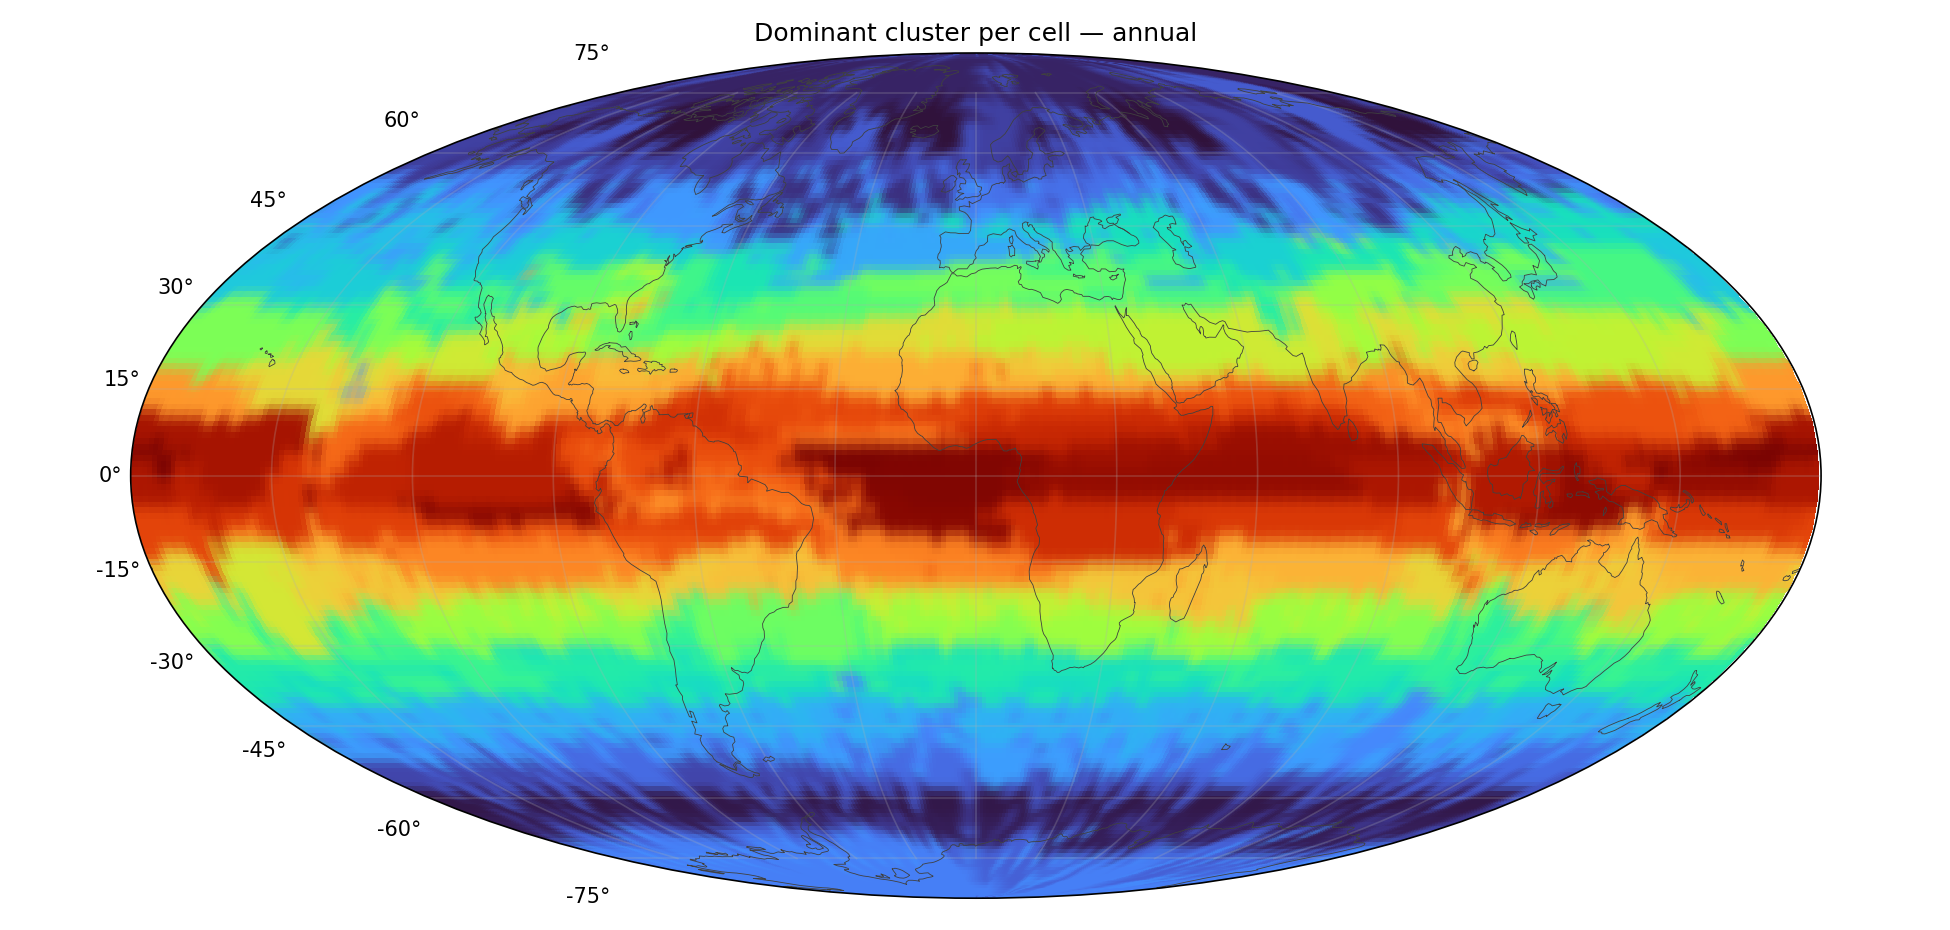
\includegraphics[width=0.74\columnwidth]{map_annual.png}
\caption{Dominant cluster per cell across the whole 2014 to 2022 record
($K{=}128$, similar clusters share hues), computed without any location
input.}
\label{fig:map}
\end{figure}
The clustering receives no location or time input, yet the dominant cluster
per cell forms contiguous regions that follow tropics, storm tracks, polar
caps and continents (Fig.~\ref{fig:map}). At raw presence level most clusters
look global, the most extreme appearing somewhere in 36\% of all cells yet
holding half its tokens in only 4.4\% of the globe. Across the run 77 of 128
clusters reach occupancy above 0.9 somewhere while 12 never pass 0.5. So
clusters have clear territories that only a threshold reveals.
A few clusters encode something specific on their own. Cluster~27 owns the
ring around the North Pole between 75 and 86$^\circ$N, the zone of retreating
sea ice, at occupancy 1.0 in its core cells. Its residual is nearly as large as
the 6-hour change itself (ratio 0.92, third highest of 128), so the encoder
gives this region its own regime but models it comparatively poorly.
Fig.~\ref{fig:terr} shows three territories spanning the range.

\subsection{Seasonality and El Ni\~no}
Seasonality is real but concentrated in a minority of clusters. The median
seasonality score (std/mean of the twelve monthly enrichments) is 0.17, and
only 35 of 128 clusters exceed 0.5, mostly winter or summer regimes. Whether
that concentration is a property of the atmosphere or partly of the method is
open. On the map, 42.8\% of cells change their dominant
cluster between DJF and JJA (Fig.~\ref{fig:season}), while the diurnal
counterpart is a null (2.6\% between 00Z and 12Z). The leading principal component of the per-date regime
mix is an almost pure seasonal harmonic ($R^2{=}0.992$). Interannual events
are visible on top of it. In the Ni\~no 3.4 box~\cite{oni}, three of the four
El Ni\~no winters of the period (2015/16, 2018/19, 2019/20, all but the weak
2014/15 event) have a mean anomaly score of 0.55 to 0.60 while four of the five
remaining winters sit at 0.12 to 0.18. The exception is the 2021/22
La Ni\~na winter at 0.52, so a high score can mark either ENSO phase. During
the record 2015/16 event the cluster that usually dominates the box drops to
its nine-year occupancy minimum.

\section{Discussion}
Both guiding questions have positive answers. Documented extremes (SSW 2018,
the above-freezing North Pole 2015, Antarctic heatwave 2022) are recoverable
from the latents as spatially and temporally coherent outlier events after
per-cell standardisation, which is needed because latent residual size is not
calibrated to physical anomaly size. Spatially the latents are organised into regimes with real territories,
visible only under a mass threshold because almost every cluster appears
somewhere on the globe. Temporally the seasonal cycle dominates and is carried by a
minority of clearly seasonal clusters, with El Ni\~no winters visible on top
of it. Occasionally a single cluster isolates a specific physical region, such
as the Arctic sea-ice ring. Finally, the latent space is a continuum with no
natural K. Its structure lies in each cluster's directions of variation
rather than in where its centre sits.

% ===================== page 3: appendix =====================
% \onecolumn, not figure* floats: a starred float can only be placed on a page
% LATER than the one it is declared on, so declaring both right after a
% \clearpage pushed them past the references onto a float page of their own.
% One column also lets the two wide maps and the reference list share one page.
\clearpage
\onecolumn
\setlength{\parskip}{2pt}

\section*{Appendix}
Both figures come from the same run as Fig.~\ref{fig:map}, on the same colours.
Regenerate with \texttt{python3 src/analysis/report\_figures.py}, which prints
every number the captions quote.

\begin{figure}[h!]
\centering
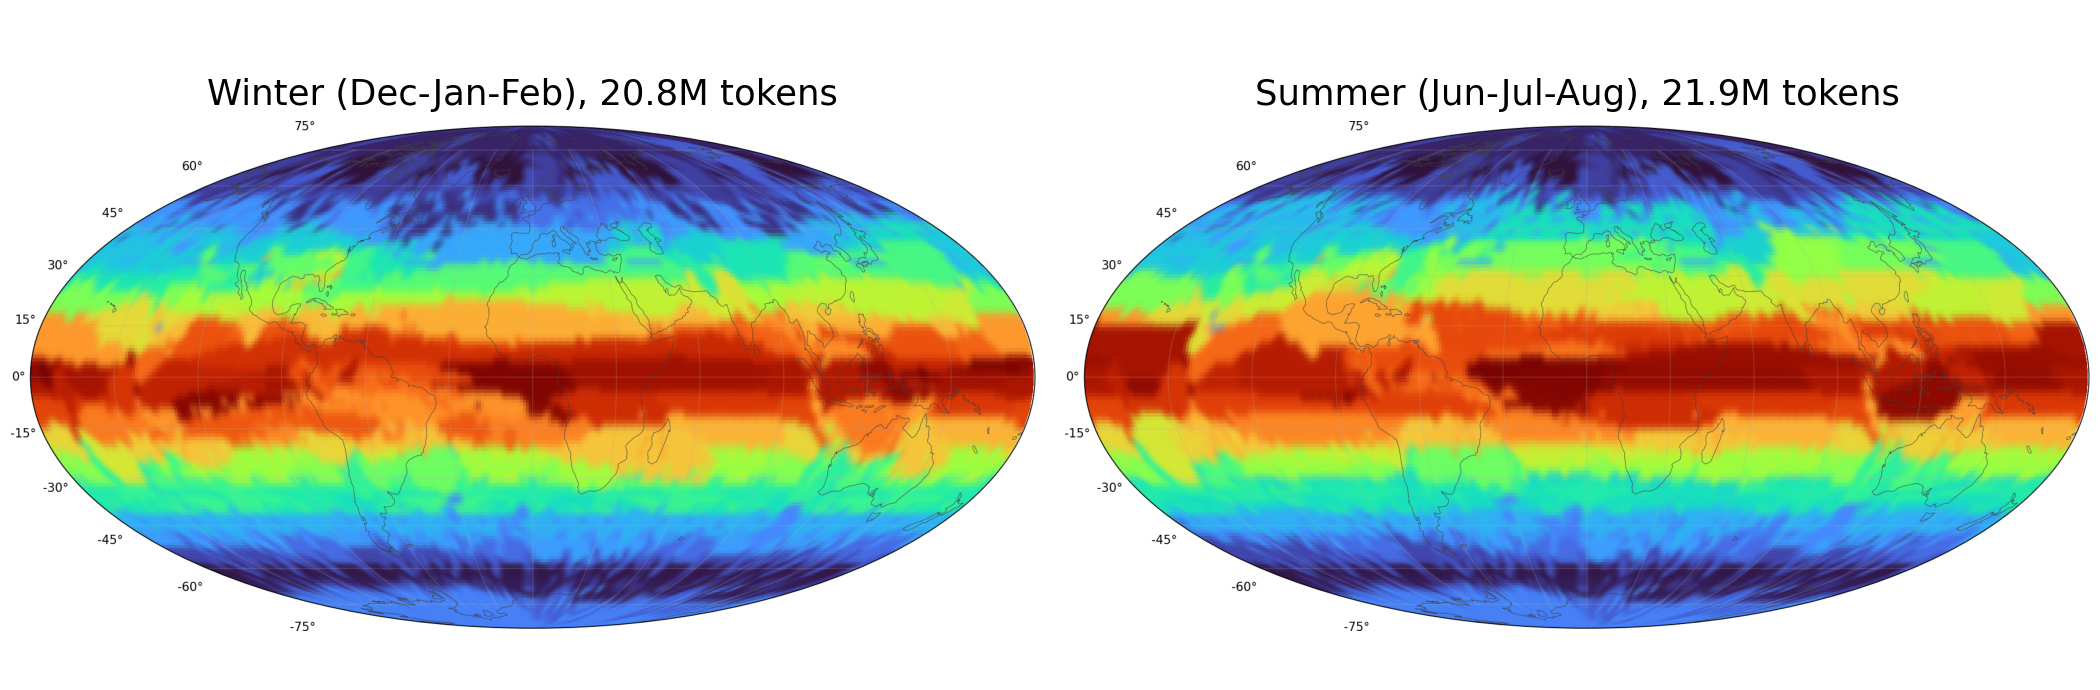
\includegraphics[width=0.76\textwidth]{fig_seasonality.png}
\caption{Dominant cluster per cell in winter and in summer (Section~3.5). A
region that keeps its colour keeps its regime. 42.8\% of cells carry a
different dominant cluster in JJA than in DJF, the tropical and northern
mid-latitude bands migrating into the summer hemisphere while the hemispheres
move in opposite phase. The diurnal version is a null, 2.6\% of cells differing
between 00Z and 12Z. December is grouped with the following January and
February.}
\label{fig:season}
\end{figure}

\begin{figure}[h!]
\centering
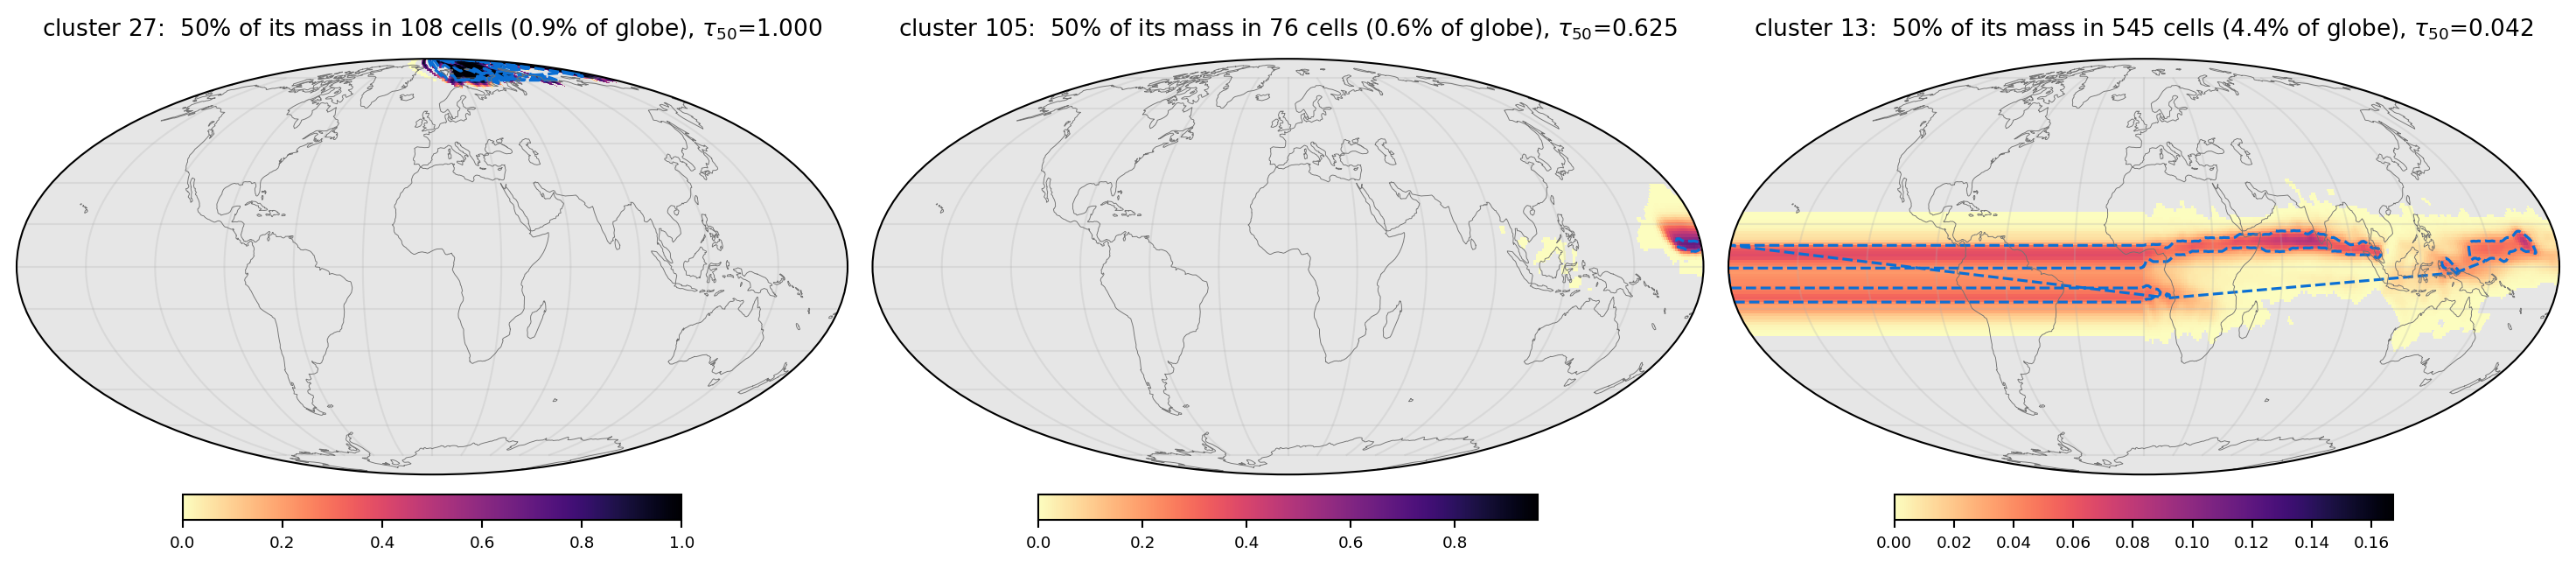
\includegraphics[width=0.94\textwidth]{fig_territories.png}
\caption{Occupancy of three clusters (Section~3.4), the fraction of the
13{,}021 time steps at which a cell carries that label. Grey marks cells the
cluster never visits and the dashed outline is the smallest set of cells
holding half the cluster's tokens. Each panel has its own colour scale because
peak occupancy is bimodal, 77 of 128 clusters peaking above 0.9 while 12 never
reach 0.5, so one shared scale would hide whichever group it missed.
Cluster 27 is a ring around the North Pole that it occupies at every time step,
cluster 105 a compact equatorial Pacific regime at the date line and the most
common label inside the Ni\~no 3.4 box, cluster 13 the run's most itinerant,
somewhere in 36\% of all cells while half its mass sits in 4.4\% of the globe.}
\label{fig:terr}
\end{figure}

\section*{References}
\vspace{-1.2\baselineskip}
\begin{multicols}{2}
\renewcommand{\refname}{}
\begin{thebibliography}{99}\scriptsize
\itemsep0pt

\bibitem{wgen} ECMWF. \emph{WeatherGenerator}. \url{https://github.com/ecmwf/WeatherGenerator}
\bibitem{era5} H. Hersbach et al. The ERA5 global reanalysis. \emph{Q. J. R. Meteorol. Soc.} 146(730):1999--2049, 2020.
\bibitem{healpix} K. M. G\'orski et al. HEALPix: a framework for high-resolution discretization and fast analysis of data distributed on the sphere. \emph{Astrophys. J.} 622(2):759--771, 2005.

\bibitem{lloyd} S. P. Lloyd. Least squares quantization in PCM. \emph{IEEE Trans. Inf. Theory} 28(2):129--137, 1982.
\bibitem{kplane} P. S. Bradley and O. L. Mangasarian. k-plane clustering. \emph{J. Global Optim.} 16(1):23--32, 2000.
\bibitem{qflat} P. Tseng. Nearest q-flat to m points. \emph{J. Optim. Theory Appl.} 105(1):249--252, 2000.
\bibitem{gonzalez} T. F. Gonzalez. Clustering to minimize the maximum intercluster distance. \emph{Theor. Comput. Sci.} 38:293--306, 1985.
\bibitem{mppca} M. E. Tipping and C. M. Bishop. Mixtures of probabilistic principal component analysers. \emph{Neural Comput.} 11(2):443--482, 1999.
\bibitem{ward} J. H. Ward. Hierarchical grouping to optimize an objective function. \emph{J. Am. Stat. Assoc.} 58(301):236--244, 1963.
\bibitem{nmi} A. Strehl and J. Ghosh. Cluster ensembles, a knowledge reuse framework for combining multiple partitions. \emph{J. Mach. Learn. Res.} 3:583--617, 2002.

\bibitem{merge} Over-cluster then merge, Section~3.2. D. Li, S. Zhou, T. Zeng and R. H. Chan, Multi-prototypes convex merging based k-means clustering, arXiv:2302.07045, 2023;
W. Qian, Y. Zhang and Y. Chen, Structures of spurious local minima in k-means, arXiv:2002.06694, 2020;
V. Menon, Gokularam M. and S. Kalyani, Subspace clustering without knowing the number of clusters, a parameter free approach, \emph{IEEE Trans. Signal Process.}, 2020, doi:10.1109/TSP.2020.3018665;
W. Li, J. Hannig and S. Mukherjee, Subspace clustering through sub-clusters, \emph{J. Mach. Learn. Res.} 22(53):1--37, 2021;
A. D. Peterson, A. P. Ghosh and R. Maitra, Merging k-means with hierarchical clustering for identifying general-shaped groups, \emph{Stat} 7(1):e172, 2018.

\bibitem{ssw2018} A. Y. Karpechko, A. Charlton-Perez, M. Balmaseda, N. Tyrrell and F. Vitart. Predicting sudden stratospheric warming 2018 and its climate impacts with a multimodel ensemble. \emph{Geophys. Res. Lett.} 45:13538--13546, 2018.
\bibitem{np2015} G. W. K. Moore. The December 2015 North Pole warming event and the increasing occurrence of such events. \emph{Sci. Rep.} 6:39084, 2016.
\bibitem{seaice2016} A. A. Petty et al. The Arctic sea ice cover of 2016, a year of record-low highs and higher-than-expected lows. \emph{The Cryosphere} 12:433--452, 2018.
\bibitem{wille2024} J. D. Wille et al. The extraordinary March 2022 East Antarctica heat wave, part I, observations and meteorological drivers. \emph{J. Climate} 37(3):757--778, 2024.
\bibitem{bw2023} E. Blanchard-Wrigglesworth, T. Cox, Z. I. Espinosa and A. Donohoe. The largest ever recorded heatwave, characteristics and attribution of the Antarctic heatwave of March 2022. \emph{Geophys. Res. Lett.} 50:e2023GL104910, 2023.
\bibitem{oni} NOAA Climate Prediction Center. \emph{Oceanic Ni\~no Index (ONI)}, cold and warm episodes by season, \texttt{cpc.ncep.noaa.gov}.

\end{thebibliography}
\end{multicols}

\end{document}
